%%%%%%%%%%%%%%%%%%%%%%%%%%%%%%%%%%%%%%%%%%%%%%%%%%%%%%%%%%%%%%%%%%%
%%% Den här mallen är skriven av Magnus Gustafsson (MG),
%%% tillämpad fysik, Luleå tekniska universitet.
%%% Den är baserad på TVM:s rapport-mall/guide i word och
%%% Lars-Göran Westerbergs latex-mall som använts i kurserna
%%% Ingenjörsvetenskap, och Ingenjörsvetenskap och rymdteknik.
%%% Om du har kommentarer eller önskemål kan du kontakta MG.
%%%%%%%%%%%%%%%%%%%%%%%%%%%%%%%%%%%%%%%%%%%%%%%%%%%%%%%%%%%%%%%%%%%

%%%%%%%%%%%%%%%%%%%%%%%%%%%%%%%%%%%%%%%%%%%%%%%%%%%%%%%%%%%%%
%%%%%%%%%%%%%%%%%%%%%%%%%%%%%%%%%%%%%%%%%%%%%%%%%%%%%%%%%%%%%
% -                  PREAMBLE STARTS HERE                 - %
%%%%%%%%%%%%%%%%%%%%%%%%%%%%%%%%%%%%%%%%%%%%%%%%%%%%%%%%%%%%%
%%%%%%%%%%%%%%%%%%%%%%%%%%%%%%%%%%%%%%%%%%%%%%%%%%%%%%%%%%%%%
%- The preamble defines the formatting of the document.

% - What is written behind the percent mark is not regarded as code. In other words, we use it to comment the code.

\documentclass{article}
\usepackage[utf8]{inputenc} % - Defines what coding LaTeX uses. Use this one.
\usepackage[english]{babel}
\usepackage{graphicx} % - Package for including images in the document.
\usepackage{caption}
\usepackage{subcaption}
\usepackage{amsmath}
\usepackage{float} % För att lägga saker exakt rätt, använd taggen [H] istället för [h] eller [h!]
\usepackage{mathtools}
\usepackage{siunitx}
\usepackage{csquotes}
\graphicspath{ {Images/} } % - Path to where the images are located
\usepackage{hyperref} % - Package for including hyperlinks in the document.
\usepackage[backend=bibtex,style=numeric,bibencoding=ascii]{biblatex}
 % - Package for the bibliography ("referenser").
\addbibresource{references.bib} % - From where the references are taken
\setlength\parindent{0pt} % - Tar bort indentering vid enter
\usepackage{svg}

% - Can be good to structure the .tex file by dividing the document using commenting. For longer documents you can create separate .tex files for each section and then include these using \import(filename.tex). For the exercise in this course it is suggested that you write everything in this main.tex file. You can of course try using \import if you like. - %

%%%%%%%%%%%%%%%%%%%%%%%%%%%%%%%%%%%%%%%%%%%%%%%%%%%%%%%%%%%%%%
% -               Title and affiliation                    - %
%%%%%%%%%%%%%%%%%%%%%%%%%%%%%%%%%%%%%%%%%%%%%%%%%%%%%%%%%%%%%%

\title{Designing an Epileptic Prediction Cap\\
\textit{Hardware, Software and Algorithms}}

\author{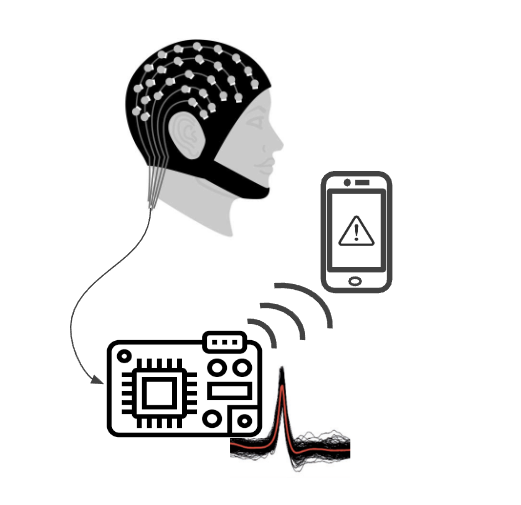
\includegraphics[width=0.6\textwidth]{images/front.png} \\ \\ \\
Author \\
{\tt Johan Axenhag johaxe-4@student.ltu.se} \\
{\tt Fabian Danielsson fabdan-8@student.ltu.se} \\
{\tt Pawel Dzialo pawdzi-7@student.ltu.se} \\
{\tt Johan Lindqvist ojaili-8@student.ltu.se} \\
{\tt Michelle von Rosen micvon-8@student.ltu.se} \\
\\Department of Computer Science, Electrical and Space Engineering \\ \\

\includegraphics[width=0.2\textwidth]{images/ltu_swe.jpg}}
% MG: Bilder på första sidan är bäst att lägga i "author"-
% kommandot såvitt jag kan se.

% Ange författare, e-post samt datum för publiceringen.
% Titelsidan kan också innehålla en figur för att locka läsaren att läsa rapporten. Figurens innehåll måste naturligtvis vara kopplat till arbetet som beskrivs i rapporten.
%
% På en titel kan man ställa höga krav. Titeln skall vara klar och beskrivande och fungera som en miniatyr-sammanfattning av arbetet. Läsaren skall förstå vad rapporten handlar om genom att läsa titeln. Trots det ska titeln vara kort, 4-12 ord, och får inte innehålla några formler, förkortningar eller speciella symboler.
%
% En bra titel är en titel som med minsta möjliga antal ord korrekt beskriver innehållet i rapporten. Det kan ibland vara praktiskt att ha en titel och en undertitel.
%
% För laborationsrapporter; E-post samt laborationshandledare skall infogas.
%
% Byt LTU logga vid engelsk rapport.

\date{\today}

\begin{document}

\maketitle
\thispagestyle{empty}% Tar bort sidnumrering, första sidan
\pagenumbering{Roman}% Romerska siffror i sidnumreringen
\setcounter{page}{0} % Bestämmer vad sidnumreringen starar på, på framsidan
\newpage
%%%%%%%%%%%%%%%%%%%%%%%%%%%%%%%%%%%%%%%%%%%%%%%%%%%%%%%%%%%%%
%%%%%%%%%%%%%%%%%%%%%%%%%%%%%%%%%%%%%%%%%%%%%%%%%%%%%%%%%%%%%
% -                  PREAMBLE ENDS HERE                   - %
%%%%%%%%%%%%%%%%%%%%%%%%%%%%%%%%%%%%%%%%%%%%%%%%%%%%%%%%%%%%%
%%%%%%%%%%%%%%%%%%%%%%%%%%%%%%%%%%%%%%%%%%%%%%%%%%%%%%%%%%%%%

%%%%%%%%%%%%%%%%%%%%%%%%%%%%%%%%%%%%%%%%%%%%%%%%%%%%%%%%%%%%%%
% -                      Abstract                          - %
%%%%%%%%%%%%%%%%%%%%%%%%%%%%%%%%%%%%%%%%%%%%%%%%%%%%%%%%%%%%%%





\section*{Abstract}
Epileptic seizures are a neurological disorder that affects surprisingly many. In this paper, an engineering approach is taken to create a prediction device. This device's goal was to predict a seizure within a 2-minute time frame while being wearable. This project was divided into three parts; EEG signal collecting hardware as well as Bluetooth communication, software that removes artifacts, and prediction algorithms that together form the complete design. Prediction algorithms were further divided into two, a spike detection and a CNN detection approach with varying results. %WRITE COMMENTS ABOUT RESULTS; ONE-TWO SENTENCE
The brain signal preprocessing was completed so that digital filters and a C library for independent components analysis were made in C. However the lack of proper experience in the neurological field made the artifact removal un-tunable for proper artifact removal.
The hardware implementation was found to be possible, but difficult because of the current silicon shortage affecting the supply chains of required components. A working prototype of an electrode along with the required amplification, filtering, and analog-to-digital conversion, and a prototype of the pre-processing, classification, and user interface device were created successfully. Testing software was also created for verifying the correctness of each data collection step in the classification procedure.
%OTHER RESULTS
In the end, a finished cap design was not achieved but rather a collection of approaches that can be used both as a foundation and also as lessons on what to avoid for further projects. The two greatest lesson's from this project, that should be considered if further studied, is that brain waves are extremely individual and how important a clear project definition is for interdisciplinary projects such as this one.

% Svenska för labrapporter.
% 
 
\newpage
%%%%%%%%%%%%%%%%%%%%%%%%%%%%%%%%%%%%%%%%%%%%%%%%%%%%%%%%%%%%%%
% -                    Table of contents                   - %
%%%%%%%%%%%%%%%%%%%%%%%%%%%%%%%%%%%%%%%%%%%%%%%%%%%%%%%%%%%%%%

\tableofcontents
\newpage

% Varje ny huvudrubrik ska börja på ny sida.
%
% Du bör ha Innehållsförteckning som rubrik till sidan. Däremot ska inte innehållsförteckningen vara en rubrik i själva innehållsförteckningen.
%
% Titelsidan skall inte sidnumreras. De sidor som får ett sidprefix på respektive sida är, förord, sammanfattning, innehållsförteckning och beteckningar. Från inledning används sidnummer.
% Sidnummer skrivs ut på respektive sida exempelvis centrerat i sidfoten. OBS sidnumrering är redan gjord i denna mall.



\newpage
%%%%%%%%%%%%%%%%%%%%%%%%%%%%%%%%%%%%%%%%%%%%%%%%%%%%%%%%%%%%%%
% -                    Introduction                        - %
%%%%%%%%%%%%%%%%%%%%%%%%%%%%%%%%%%%%%%%%%%%%%%%%%%%%%%%%%%%%%%
\pagenumbering{arabic}% Arabiska siffror i sidnumreringen
\setcounter{page}{1} % Sätter sidnumreringen till 1 på denna sida
\section{Introduction}
Inledningen introducerar läsaren till problemställningen och ger bakgrunden till problemet. Inledningen är viktig för det är här som läsaren skall ledas in i hur författaren tänkt. Hela avsnittet bör skrivas så att läsaren logiskt och motiverat leds fram till den problemställning som rapporten behandlar. I inledningen skall det finnas en översikt över närliggande tidigare arbeten inom ämnet. Även här gäller att göra läsaren intresserad så att hen läser vidare i rapporten. Slutklämmen i inledningen bör göras så att det blir en mjuk övergång från Inledning till nästa kapitel.



Här kan vara exempel med numrerade referenser: ''kan beskrivas enligt \cite{Sterte2001}''.
Ge syftet med arbetet dvs vad som vill åstadkommas med arbetet, frågeställningar och vilka avgränsningar som finns. Målen skall vara specifikt klarlagda samt i rapportens slutsatser ska det tydligt framgå hur målen uppnåtts.

% Kan med fördel indelas i underrubriker; Bakgrund, Problemformulering, Litteraturstudie,
% Syfte och mål, Avgränsningar.
%
% Lite skriv-vett
%
% 1. Använd aktiv form (vattnet strömmade genom röret). Det gör rapporten mer livlig.
% 2. Använd dåtid för observationer mm. Exempelvis ”ökat tryck gav större flöde”.
% 3. Använd nutid för generaliseringar och allmänt giltiga påståenden. Exempelvis
% ”I de flesta fall tillhör problemen kategorin olösbara problem”.
% 4. Undvik strunt, pompösa meningar och alla överdrifter. Uttryck som ``utmärkt
% överenstämmelse'' eller ``fantastisk mätnoggrannhet'' får inte förekomma.
% 5. Samtliga tidigare arbeten som åberopas i rapporten skall refereras.
% 6. Skriv inte rapporten som en berättelse om vad ni gjort.
% 7. Berätta inte om de idéer som inte gav något.
% 8. Var mycket försiktig med negativa kommentarer om det egna arbetet.




%%%%%%%%%%%%%%%%%%%%%%%%%%%%%%%%%%%%%%%%%%%%%%%%%%%%%%%%%%%%%%
% -                       Theory                           - %
%%%%%%%%%%%%%%%%%%%%%%%%%%%%%%%%%%%%%%%%%%%%%%%%%%%%%%%%%%%%%%
\newpage
\section{Theory}

%A sense of unease, a distance to world around me, then a sudden lack of control, my body no longer obeys, soon the seizure will come. This is the feeling for some people who suffer from epileptic seizure, but for some there is no warning, no foreboding feeling, only a sudden seizure. Epilepsy is a neurological disorder that is affecting around 50 million people world wide 
%[https://www.who.int/news-room/fact-sheets/detail/epilepsy#:~:text=Epilepsy]
%. In this work we aim to provide that warning to those 50 million, thus improving their quality of life. We are not the first to atempt this, there has been a great deal of interest in the area of epileptic prediction and warning in recent years. 
%kolla den rapport som sammanställer

%As far as the current devices go they mostly aim at detecting sudden and unsuspected movement, whic 
%The system we propoce is that of a wearable hat, equiped whit electrodes that can detect EEG signals, whic then is runned through a Neural Network that detects the so called preictal state that precedes the epileptic seizure.

% Med figurer avses bilder, diagram, grafer mm. Det ska inte finnas ytterligare rubrik
% i figuren än den som står i figurtexten. Om ej egentillverkad skall källa anges samt
% tillstånd av ägare erhållas.
%
% Variabler skrivs kursivt både i ekvationerna och i brödtexten. Icke-variabler skrivs på vanligt sätt.
% Ekvationer betraktas som en del i texten. Ekvationsnummer ska skrivas längst ut till höger.

\subsection{Literature review}

\subsection{Epileptic seizures}
A (epileptic) seizure can be conceptualized as occurring when there is distortion of the normal balance between excitation (E) and
inhibition (I) in the brain (Stafstrom and Carmant, 2022, p. 3). In practice however this imbalnance can be expressed in a multidues of ways ranging from spasms, loss of consciousness and secondary injuries given from for example when repeatedly hitting hard surfaces with the head.
The seizure onset can be differantiated into four epileptic brain states, the Interictal state, the Preictal state, the Ictal state and the Post-ictal state.
The Interictal state is the "normal state" or when no seizure are present or on the way. The preictal state is just before seizure onset while The Ictal state is during the seizure onset. The Post-ictal is the state jus after the seizure and eventually fades out into a new Interictal state. 
There has been many studies discussing the existance of a preictal state but after the results of Lehnertz (2001), where changes just before seiuzure onset could be clearly seen, it has been regarded as a "proof of concept of the existence of a preictal state" Gadhoumi et al.(2015).
Seizure prediction cane be considered as early detection of the preictal state (Bou Assi et al, 2017, p. 1) which also is the goal of this project.

\subsection{Prediction}

\subsubsection{Dataset}

\subsubsection{Feature extraction}

\subsubsection{Prediction algoritm}
% Måste inte ha egen rubrik utan kan ingå i teorins löpande text.
% I fall teorikapitlet utelämnas ska litteraturstudie ingå i inledningen.




%%%%%%%%%%%%%%%%%%%%%%%%%%%%%%%%%%%%%%%%%%%%%%%%%%%%%%%%%%%%%%
% -                       Method                           - %
%%%%%%%%%%%%%%%%%%%%%%%%%%%%%%%%%%%%%%%%%%%%%%%%%%%%%%%%%%%%%%
\section{Method}
%Kan i vissa fall delas upp i metodbeskrivning, experimentell uppställning och arbetsgång. Att redogöra för sin metod är viktigt bland annat för att förklara varför den valda metoden ger ett tillförlitligt resultat. Alla antaganden och förenklingar måste anges och motiveras. Definiera matematiska modeller så att andra ingenjörer och forskare kan förstå vad du gjort.
%Exempelvis utnyttjades Microsoft Excel 2013 för att analysera mätresultaten och plotta mätdata.

% Här beskrivs metoden, ofta är det lämpligt att dela upp texten i ett antal underrubriker.
% Använd alltid högst tre rubrik-nivåer.
\subsection{Dataset}
For training purposes the CHB-MIT dataset was used. This dataset was recorded at the Boston children hospital on $22$ patient of ages $1.5 - 19$. The dataset was published the $9th$ of june $2010$. The dataset is split into $23$ cases (one for each patient except $2$ that were for the same patient) numbered as chb$1$ to chb$23$. A case contains between $9$ and $42$ files containing roughly $23$ EEG signals, whit a resolution of $16$-bit these were sampled at a rate of $256$ samples per second.


\subsection{Experimental setup}

%Alla eventuella försöksuppställningar beskrivs på ett sådant sätt att andra kan upprepa samma försök och verifiera dina resultat. Utnyttja figurer som förenklar din beskrivning.




%%%%%%%%%%%%%%%%%%%%%%%%%%%%%%%%%%%%%%%%%%%%%%%%%%%%%%%%%%%%%%
% -                      Results                           - %
%%%%%%%%%%%%%%%%%%%%%%%%%%%%%%%%%%%%%%%%%%%%%%%%%%%%%%%%%%%%%%
\section{Result}
% Innehåll: resultat och analys.
% I vissa fall kan man ha ”Resultat och diskussion” som kapitel.

%Detta är förmodligen den största delen av rapporten. Här redovisas resultaten rakt på sak på ett objektivt/neutralt sätt. Ofta är det lämpligt att dela upp texten i ett antal underrubriker. Materialet måste presenteras i logisk ordning, vilket inte behöver vara den ordning i vilken försöket/arbetet har utförts.

%Läsaren skall kunna läsa rapporten utan att behöva bläddra fram och tillbaka. Det ska vara tydligt vad som är data respektive analys av data.
%Visas resultat i tabell- eller figurform så måste kortfattat beskrivas vad man ser i figurerna/tabellerna. De placeras i närheten (efter) där de först refererades.

%Som exempel visas fyra mätningar där variabel, 1, varierades. Resultat visas i tabell \ref{tvariabel123} nedan.

% Det skall alltid finnas en tabelltext som förklarar vad som finns i tabellen. Tabellnummer och text ska stå ovanför tabellen.
\subsection{Spike based algorithms}
The algorithm was tested on 8 recordings from three patients, whit a derivative threshold tuned by analysis of the interictal period. The resulting predictions and their accuracy can be seen in the tables(\ref{Der1}-\ref{Der3})

%for the first patient, the algorithm got a precision of $0.33$, a miss rate of $0$, and sensitivity of $1$.The second patient had 


\begin{table}[H]
\centering
    \begin{tabular}{c | c |c |c | c}
        \hline
         file &  FP (timestamps) & TP (timestamps) & NP (timestamps) & (seizure time)  \\
        \hline
        chb1-01 & (180) & Null & Null & Null   \\
        chb1-02 & (180,1620) & Null & Null & Null \\
        chb1-03 & Null & (2160,2520,2700) & Null & (2996)
        \\
        chb1-04	&  Null &   (1260) & Null & (1467)\\
        chb1-05 &   (360,1620) & Null & Null & Null\\
        chb1-06 &   (1440) & Null & Null & Null\\
        chb1-07 &   (1260,900) & Null & Null & Null  \\
        chb1-08 &   (1260) & Null & Null & Null  \\
        \hline
     \end{tabular} 
\caption{Patient number 1, whit criteria set as $2< der < \infty$ }
\label{Der1}
\end{table}

\begin{table}[H]
\centering
    \begin{tabular}{c | c |c |c | c}
        \hline
         file &  FP (timestamps) & TP (timestamps) & NP (timestamps) & (seizure time)  \\
        \hline
        chb2-01 & Null & Null & Null  & Null  \\
        chb2-02 & Null & Null & Null & Null \\
        chb2-03 & Null & Null & Null & Null  \\
        chb2-04	& Null & Null & Null & Null\\
        chb2-05 & Null & Null & Null & Null\\
        chb2-06 & (180,360,1620) & Null & Null & Null\\
        chb2-07 &  Null & Null & Null & Null  \\
        chb2-08 &  Null & Null & Null & Null  \\
        \hline
     \end{tabular} 
\caption{Patient number 2, whit a criteria set as $2< der < \infty$ }
\label{Der2}
\end{table}


\begin{table}[H]
\centering
    \begin{tabular}{c | c |c |c | c}
        \hline
         file &  FP (timestamps) & TP (timestamps) & FN (timestamps) & (seizure time)  \\
        \hline
        chb3-01 & (375) & Null & (362)  & (362)  \\
        chb3-02 & (1080) & (360,720) & Null & (731) \\
        chb3-03 & (1080,1260,1440,1980)& Null & (432) & (432)  \\
       chb3-04	& Null & (180), & Null & (2162)\\
        chb3-05 & Null & Null & Null & Null\\
        chb3-06 & Null & Null & Null & Null\\
        chb3-07 &  Null & Null & Null & Null  \\
        chb3-08 &  Null & Null & Null & Null  \\
        \hline
     \end{tabular} 
\caption{Patient number 3, whit a criteria set as $-0.03< der < 0.05$ }
\label{Der3}
\end{table}


The spike frequency method was tuned by measuring the maximum interictal period across all channels in the first seizure free file of the respective patient. The result is shown in the tables(\ref{Freq1}-\ref{Freq6}).Note that some of the false positives is not a true miss,it hits the seizure, it is merely that it failed to predict it. The maximum spike frequency of the inter-ictal period was aproximately $1.2857$ for patient 1, $3.5714$ for patient 2 and $0.85714$ for patient 3.

\begin{table}[H]
\centering
    \begin{tabular}{c | c |c |c | c}
        \hline
         file &  FP (timestamps) & TP (timestamps) & NP (timestamps) & (seizure time)  \\
        \hline
        chb1-01 & Null & Null & Null  & Null  \\
        chb1-02 & Null & Null & Null & Null \\
        chb1-03 & (3020) & (2995) & Null & (2996) \\
        chb1-04	& (1470) & Null & (1467) & (1467)\\
        chb1-05 & Null & Null & Null & Null\\
        chb1-06 & Null & Null & Null & Null\\
        chb1-07 &  Null & Null & Null & Null  \\
        chb1-08 &  Null & Null & Null & Null  \\
        \hline
     \end{tabular} 
\caption{Patient number 1, with a criteria set as $Spike frequency > 1.2857*1.3$ }
\label{Freq1}
\end{table}
%2.714

\begin{table}[H]
\centering
    \begin{tabular}{c | c |c |c | c}
        \hline
         file &  FP (timestamps) & TP (timestamps) & NP (timestamps) & (seizure time)  \\
        \hline
        chb1-01 & Null & Null & Null  & Null  \\
        chb1-02 & Null & Null & Null & Null \\
        chb1-03 & (805) & (1135) & Null & (2996) \\
        chb1-04	& Null & (1460,1465) & Null & (1467)\\
        chb1-05 & Null & Null & Null & Null\\
        chb1-06 & Null & Null & Null & Null\\
        chb1-07 &  Null & Null & Null & Null  \\
        chb1-08 &  Null & Null & Null & Null  \\
        \hline
     \end{tabular} 
\caption{Patient number 1, with a criteria set as $Spike frequency > 1.2857*1.1$ }
\label{Freq2}
\end{table}

\begin{table}[H]
\centering
    \begin{tabular}{c | c |c |c | c}
        \hline
         file &  FP (timestamps) & TP (timestamps) & NP (timestamps) & (seizure time)  \\
        \hline
        chb2-01 & Null & Null & Null & Null  \\
        chb2-02 & Null & Null & Null & Null \\
        chb2-03 & Null & Null & Null & Null  \\
        chb2-04	& Null & Null & Null & Null\\
        chb2-05 & Null & Null & Null & Null\\
        chb2-06 & Null & Null & Null & Null\\
        chb2-07 &  Null & Null & Null & Null  \\
        chb2-08 &  Null & Null & Null & Null  \\
        \hline
     \end{tabular} 
\caption{Patient number 2, with a criteria set as $Spike frequency > 3.5374*1.3$ }
\label{Freq3}
\end{table}

\begin{table}[H]
\centering
    \begin{tabular}{c | c |c |c | c}
        \hline
         file &  FP (timestamps) & TP (timestamps) & NP (timestamps) & (seizure time)  \\
        \hline
        chb2-01 & Null & Null & Null & Null  \\
        chb2-02 & Null & Null & Null & Null \\
        chb2-03 & Null & Null & Null & Null  \\
        chb2-04	& Null & Null & Null & Null\\
        chb2-05 & Null & Null & Null & Null\\
        chb2-06 & Null & Null & Null & Null\\
        chb2-07 &  Null & Null & Null & Null  \\
        chb2-08 &  Null & Null & Null & Null  \\
        \hline
     \end{tabular} 
\caption{Patient number 2, with a criteria set as $Spike frequency > 3.5374*1.1$ }
\label{Freq4}
\end{table}

\begin{table}[H]
\centering
    \begin{tabular}{c | c |c |c | c}
        \hline
         file &  FP (timestamps) & TP (timestamps) & NP (timestamps) & (seizure time)  \\
        \hline
        chb3-01 & (375,395) & Null & (365) & (365)  \\
        chb3-02 & (755,760) & Null & (731) & (731) \\
        chb3-03 & (445,450,460) & (85,430) & Null & (432)  \\
        chb3-04	& (2170) & Null & (2162) & (2162)\\
        chb3-05 & Null & Null & Null & Null\\
        chb3-06 & Null & Null & Null & Null\\
        chb3-07 &  Null & Null & Null & Null  \\
        chb3-08 &  Null & Null & Null & Null  \\
        \hline
     \end{tabular} 
\caption{Patient number 3, with a criteria set as $Spike frequency > 0.85714*1.3$ }
\label{Freq5}
\end{table}

\begin{table}[H]
\centering
    \begin{tabular}{c | c |c |c | c}
        \hline
         file &  FP (timestamps) & TP (timestamps) & NP (timestamps) & (seizure time)  \\
        \hline
        chb3-01 & (375) & Null & (365) & (365)  \\
        chb3-02 & (755,760) & Null & (731) & (731) \\
        chb3-03 & (450,445,460) & (85,430) & Null & (432)  \\
        chb3-04	& (2170) & Null & (2162) & (2162)\\
        chb3-05 & Null & Null & Null & Null\\
        chb3-06 & Null & Null & Null & Null\\
        chb3-07 &  Null & Null & Null & Null  \\
        chb3-08 &  Null & Null & Null & Null  \\
        \hline
     \end{tabular} 
\caption{Patient number 3, with a criteria set as $Spike frequency > 0.85714*1.1$ }
\label{Freq6}
\end{table}



%Med hjälp av mätvärdena i tabell 1 skapas en produktansats av typen potensfunktion
% där $C, \alpha, ..., \delta$ är konstanter som ska bestämmas experimentellt.
% Avgiven värmemängd från brödrosten (variabel 3) som funktion av tiden variabel 1 visas i figur \ref{fvariabel3vs1}. Den linjära anpassningen i figuren visar att

% och tillförd värmeeffekt till brödrosten bestäms då till 351,8 W.

% Diagram ska ha storhet och enhet på axlarna (SI). Är det tex logaritmerade diagram
% ska de ha storhet (men inte enhet) på axlarna. Figurnummer och text ska stå under
% figur och hänga ihop på samma sida.




\subsection{CNN}



%Neural network (notes)

%70-80\% accuracy on test set

%still not working properly on a continuous stream of data

%works somewhat ok on the continuous data on timeframes from which training data was drawn.

%does not work across multiple occasions or across multiple people, which means that the model isn't general enough, but it still adapts to the existing dataset

%why is that?

%likely because the model is adapting to the noise difference of the different occasions, and that is apparently more prevalent than the difference in states.

%Vad är då vårt resultat?

%Jo, med väldigt hög pricksäkerhet, ofta över 75\%, lyckas nätverket gissa på aldrig tidigare sedd data från test-settet. Det är ju helt fantastiskt, och allt som återstår nu är att testa nätverket i ett “riktigt” scenario, där vi kontinuerligt kör nätverket över en hel session och försöker förutspå ett stundande anfall. Funkar det?

%Nja, kanske. Här syns inget tydligt sammanhang förutom 5 minuter innan anfallet, och detta är “nedsmutsade” resultat, då denna instans av nätverket har fått träna på data från dessa 5 minuter.

%Intressantare vore att göra om datasettet men exkludera dessa 2 anfall.

%Och det kan vi se här. Detta är legitima resultat, men problemet är att det inte längre går att se någon tydlig indikation på att ett anfall är på väg att hända, i alla fall inte inom de tidsramar som vi satt. Men, som vi har plottat det nu så är det vikten för pre-iktalt stadie minus vikten för inter-iktalt stadie. Plotten ger alltså positivt när nätverket tror att en anfall ska ske, och negativt när det inte tror det. Här kommer bilder på sessioner där inget anfall skett.

%Intressant nog så är gissningen nära noll på ena, och kraftigt negativ på andra. Är detta en indikation på att nätverket fungerar? Det är svårt att säga. Hur som helst fungerar det inte som vi förväntar oss att det ska fungera, åtminstone inte inom samma tidsram.

%Slutligen kan vi konstatera att just detta nätverk inte fungerar på nästa patient. Här ser vi individualiteten in action, gissningen verkar helt omvänd.

The CNN is trained on a dataset that contains over 20 hours of data from patient chb1 from the CHB-MIT dataset, compressed into 43200 labelled datawindows. The network was trained and retrained many times with slight modifications. \\

The network has a high accuracy on the test set, about often above 75\%. This means that the network successfully adapts to the dataset, and can predict the epileptic states of the never before seen test set with high accuracy. \\

To further investigate, a simulated scenario meant to represent real life was set up. This works by taking the prediction for pre-ictal, and subtracting the prediction for inter-ictal, and then averaging over time. This yields a graph that can be investigated to visually determine the performance of the network. \\

At first, the simulated scenarios were done on data from the same EEG sessions that the network trained on. The results of that can be seen in figure (\ref{pre_both}).

\begin{figure}[H]
\centering
\begin{subfigure}{0.5\textwidth}
  \centering
  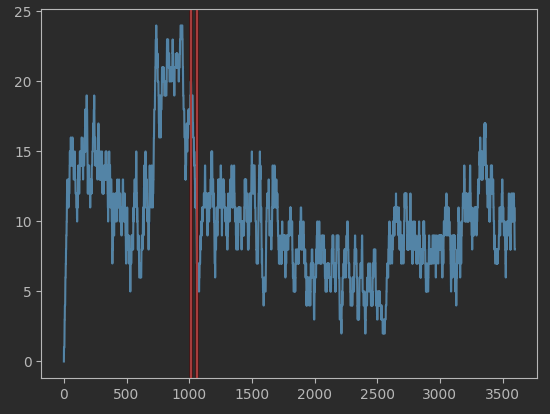
\includegraphics[width=0.9\textwidth]{images/f1-1.png}
  \caption{}
  \label{pre_sub1}
\end{subfigure}%
\begin{subfigure}{0.5\textwidth}
  \centering
  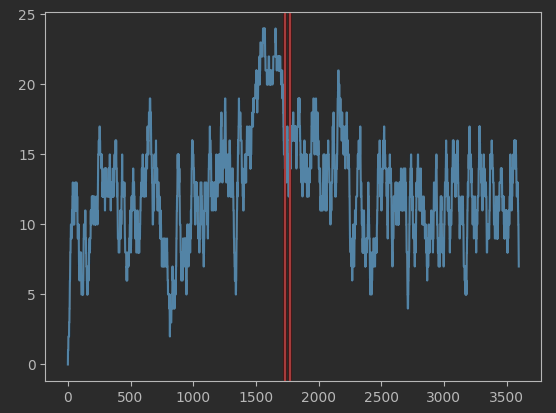
\includegraphics[width=0.9\textwidth]{images/f1-2.png}
  \caption{}
  \label{pre_sub2}
\end{subfigure}
\caption{The results of running a trained network through a simulated scenario meant to represent real life, using data that has been trained on.}
\label{pre_both}
\end{figure}

The result from figure (\ref{pre_both}) clearly increases before the seizure, but it is not presentable as a ``real" result, since it uses data from the same occasions both in the training and to validate itself. To get a proper test, the network has to be retrained on a new dataset, omitting the occasions that will later be used for the visual validation. The results of that can be seen in figure (\ref{real_both}).

\begin{figure}[H]
\centering
\begin{subfigure}{0.5\textwidth}
  \centering
  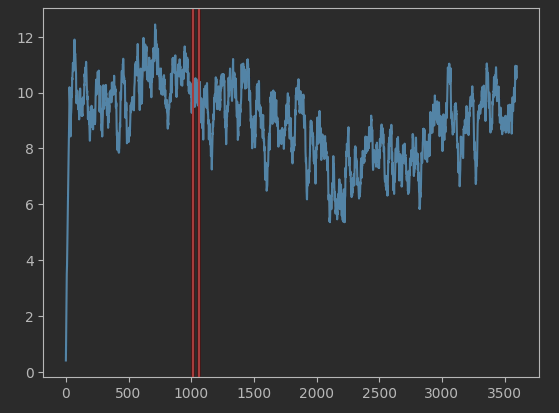
\includegraphics[width=0.9\textwidth]{images/f2-1.png}
  \caption{}
  \label{real_sub1}
\end{subfigure}%
\begin{subfigure}{0.5\textwidth}
  \centering
  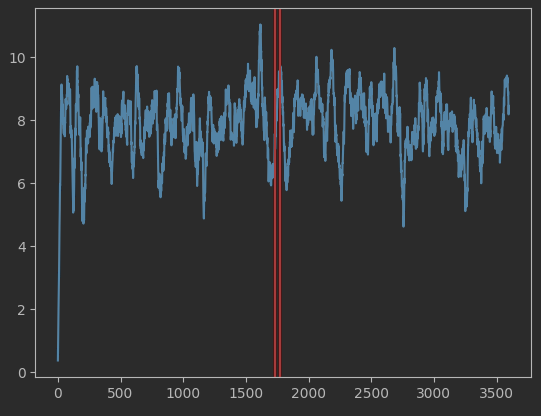
\includegraphics[width=0.9\textwidth]{images/f2-2.png}
  \caption{}
  \label{real_sub2}
\end{subfigure}
\begin{subfigure}{0.5\textwidth}
  \centering
  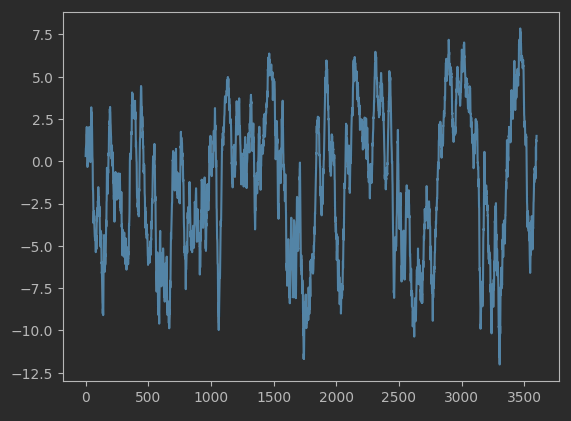
\includegraphics[width=0.9\textwidth]{images/f2-3.png}
  \caption{}
  \label{real_no_sub1}
\end{subfigure}%
\begin{subfigure}{0.5\textwidth}
  \centering
  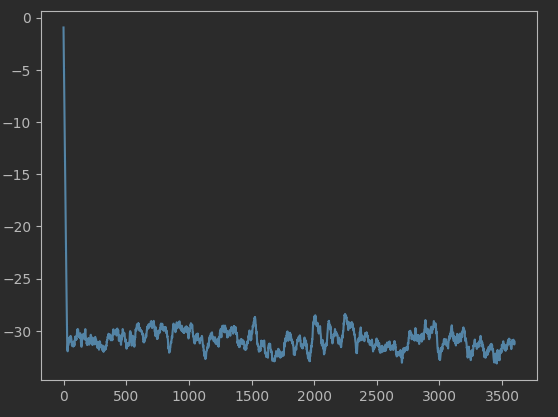
\includegraphics[width=0.9\textwidth]{images/f2-4.png}
  \caption{}
  \label{real_no_sub2}
\end{subfigure}
\caption{The results of running a trained network through a simulated scenario meant to represent real life, without using data that has been trained on.}
\label{real_both}
\end{figure}

As can be seen in figure (\ref{real_both}), when putting the network into this ``real" scenario, the network stops performing well. Instead of seeing an increasing amount of predictions for pre-ictal states closer to the seizure, the prediction distribution seems to be relatively stable throughout the test. However, a pattern still emerges. In data collection occasions where a seizure did occur, the average prediction sum seems much higher than in the occasions where no seizures occurred. \\

For a final test, the network was tested on another patient, chb03 from the CHB-MIT dataset. The results can be seen in figure (\ref{other_both}).

\begin{figure}[H]
\centering
\begin{subfigure}{0.5\textwidth}
  \centering
  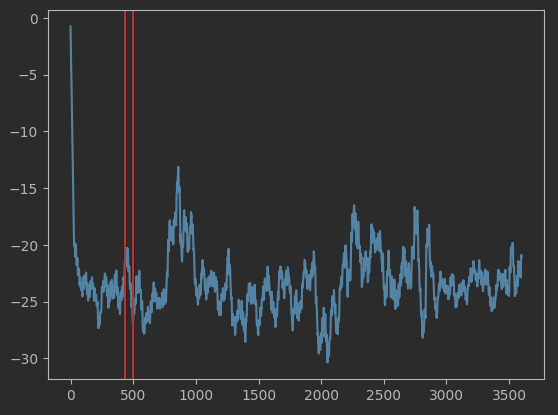
\includegraphics[width=0.9\textwidth]{images/f3-1.png}
  \caption{}
  \label{other_sub1}
\end{subfigure}%
\begin{subfigure}{0.5\textwidth}
  \centering
  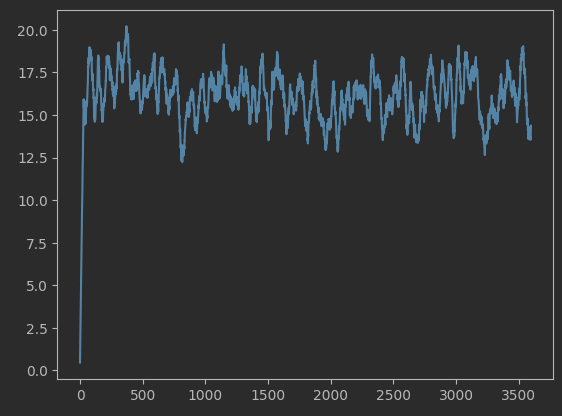
\includegraphics[width=0.9\textwidth]{images/f3-2.png}
  \caption{}
  \label{other_sub2}
\end{subfigure}
\caption{The results of running a trained network through a simulated scenario meant to represent real life, run on another patient than the one trained on.}
\label{other_both}
\end{figure}

The results from figure (\ref{other_both}) are the exact opposite of what was expected. The network predicts inter-ictal throughout a test occasion where a seizure is happening and pre-ictal throughout a test occasion where no seizure occurs. This is a clear indication that the network does not work on a patient it has not trained on.

\subsection{Hardware}
The data processing board from the figure (\ref{fig:PCBData}) in Appendix(\ref{circpart}) is tested in a simulation environment and performs as expected. It is tested with the spike detection algorithm and gets the same result as if it were run on a computer. The UART communication works, but it seems to be some error with the digital isolator, which we have not been able to solve. Assessment of the rest of the circuitry from Appendix(\ref{circpart}) is done both in simulation when possible and primarily by building the circuits on a breadboard and testing them individually. Figure (\ref{fig:ampsim}) shows a simulation plot of the amplification. An input of \SI{10}{\micro\volt} is used, and it produces an output with a max amplitude of \SI{130}{\milli\volt}, which should be sufficient for the ADCs. The amplifier is also tested using a PI-attenuator and a signal generator to test the circuitry with signals in the desired range. From the test, it can be concluded that the amplifier works as intended, but tuning the gain by varying $R_G$ or adding more gain to the buffer stage could be needed, but it needs to be tuned in on the final circuit. All the filters are tested in the same manner and perform as expected. Sadly, the state of the current semiconductor market and delays made it impossible to finish the final circuit at the time of the project course, so no final test with the electrode was run. But since all stages except for the ADCs, which did not arrive in time, are tested separately and work, it is reasonable to assume that the current designs should work but would perhaps need some tuning to get optimal readings.
\begin{figure} [H]
\begin{center}
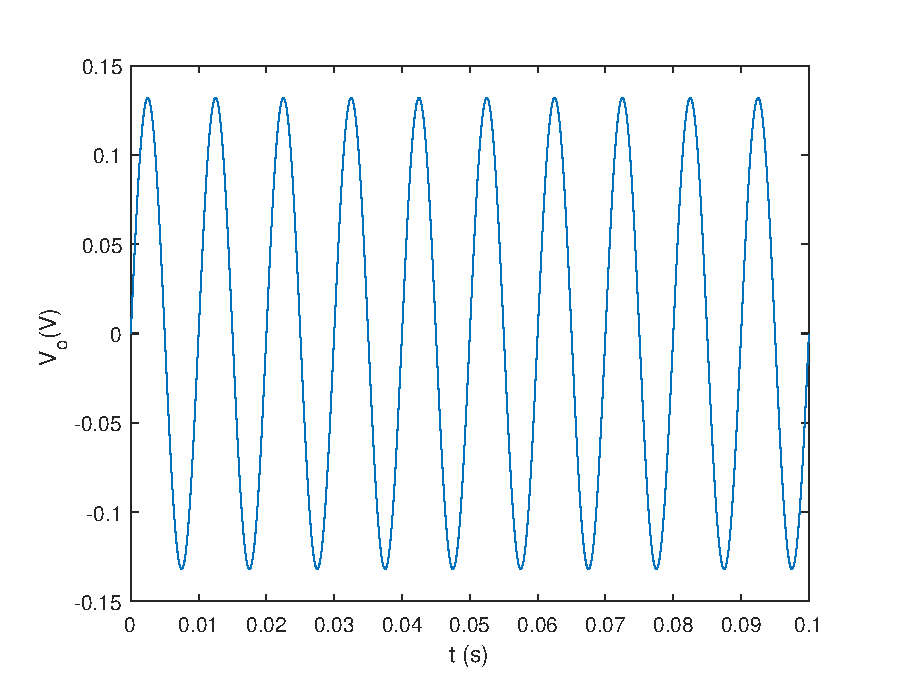
\includegraphics[scale=0.8]{images/Ampout.eps}
   \caption{Simulation of instrumentation amplifier with a input of \SI{10}{\micro\volt}}
    \label{fig:ampsim}
\end{center}
\end{figure}









%%%%%%%%%%%%%%%%%%%%%%%%%%%%%%%%%%%%%%%%%%%%%%%%%%%%%%%%%%%%%%
% -                      Summary                           - %
%%%%%%%%%%%%%%%%%%%%%%%%%%%%%%%%%%%%%%%%%%%%%%%%%%%%%%%%%%%%%%
\section{Discussion and Conclusions}
% Kan delas i separata kapitel: ”Diskussion” respektive ”Slutsatser”. Slutsatser skall vara korta och koncisa.
% Ibland är det lämpligast med indelningen ”Diskussion” samt ”Slutsatser och fortsatt arbete”

%Här diskuteras (vad betyder/medför) resultaten utifrån ett vidare perspektiv och ställs i relation exempelvis till tidigare arbeten, referera i sådant fall till dessa. Utgående härifrån dras nödvändiga slutsatser som ska svara på de mål som angivits och vad resultaten har för relevans. Koppla slutsatser till uppställda mål.

%Diskutera felkällor och osäkerheter.
%Det är även lämpligt att i denna del avsluta med förslag och rekommendationer på fortsatta studier och undersökningar i ämnet. Man kan dela upp diskussion, slutsatser och framtida studier i fristående kapitel.

\newpage
\appendix
%\section{Team members}
%%Short summary of team members and what you have done in the project
%\subsection{Pawel Dzialo}
%Responsible mostly for the software implementation on the MCU, as well as the simulator, and the Android app. Also had his hand in the spike detection algorithms, a small contribution to the CNN with a CHB-MIT database file reader, and some contribution to the hardware design, mostly the ADC multiplexing part, and some ideas for the overall PCB.

%\subsection{Fabian Danielsson}
%Responsible for making and training the CNN, with everything that entailed. That includes making the dataset, and through that also making the dataset generator that was used.

%\subsection{Johan Lindqvist}
%I am currently studying my last year of Engineering Physics and Electrical engineering. My main areas of interest are Control theory, Dynamical systems and signal processing. Basically, I love mathematics and its application to control, estimate or analyse systems. Due to these tendencies, I was set to work on the prediction algorithm, Did some initial work on machine learning but then shifted to completely focus on spike prediction methods. Collaborated with Pawel Dzialo on a spike frequency algorithm and then worked on improving these results, mainly by the Derivative based method proposed in this paper, as well as a matching filter in order to increase the accuracy of the spike frequencies.

%\subsection{Johan Axenhag}
%I currently study Engineering Physics and Electrical engineering with a master's in Electrical systems and Control engineering. For this project, I have mainly been involved with the electronics part with responsibility for the hardware both in designing the circuits for the data acquisition and for the data processing. During the first half of the course, most of the time was spent trying to understand the current hardware and finding components that could be used to achieve a similar result. During the second part of the course, most time went into designing and testing the different circuits. Additionally, finding and ordering parts was an additional responsibility.
\section{Circuits}\label{circpart}
%Images of the complete circuits and PCBs
\subsection{Schematics}
Below is a presentation of the central schematics for the circuitry. In all cases where a power pin is used, a decoupling capacitor of 100nF is used. The schematics are presented in separate parts since the whole project is too large to get a good image of the complete system.
\begin{figure} [H]
\begin{center}
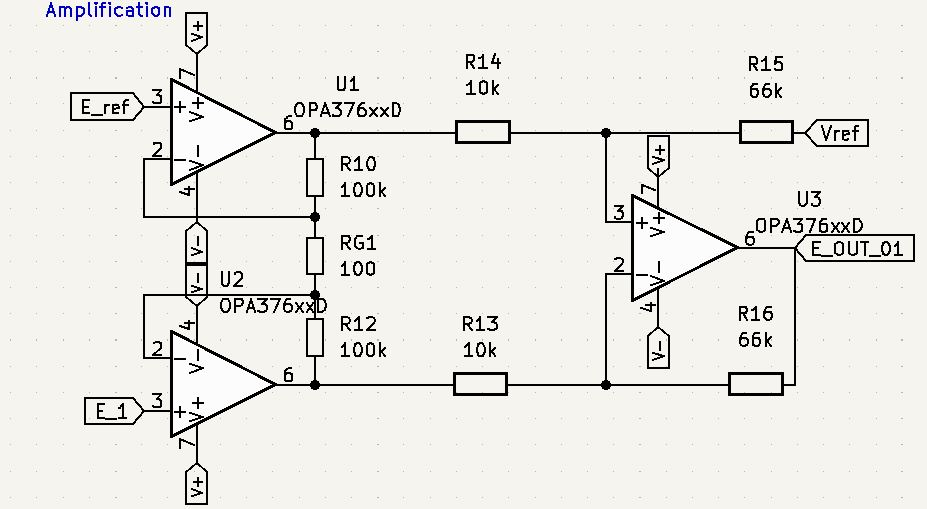
\includegraphics[scale=0.5]{images/Amplifiern.jpg}
   \caption{Instrumentation amplifier used to amplify the electrode signal and to suppress common mode noise}
    \label{fig:amplifier}
\end{center}
\end{figure}

\begin{figure} [H]
\begin{center}
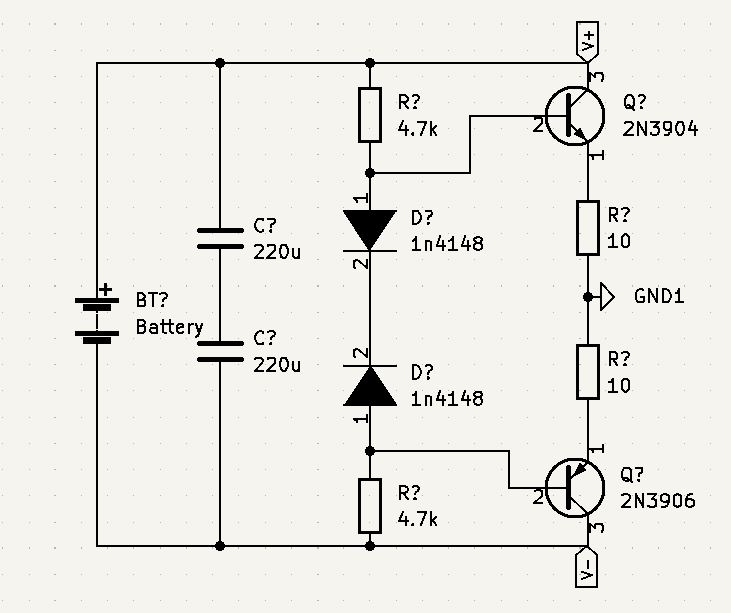
\includegraphics[scale=0.5]{images/Railsplitter.jpg}
   \caption{Rail splitter circuit designed after Sijosae Discreet Rail Splitter design \cite{railsplit}}
    \label{fig:railsplit}
\end{center}
\end{figure}

\begin{figure} [H]
\begin{center}
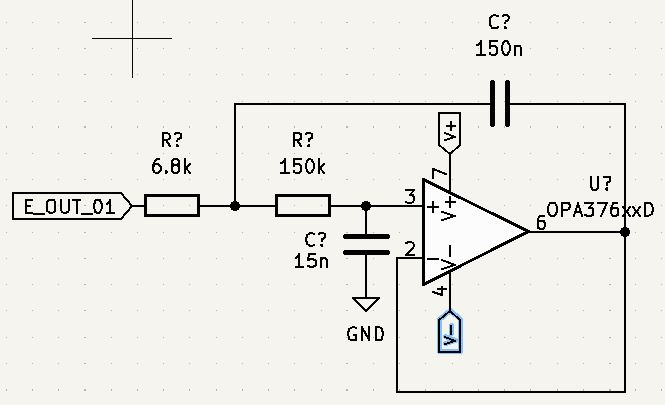
\includegraphics[scale=0.65]{images/Antialiasing.jpg}
   \caption{Second order Sallen-Key lowpass Butterworth filter used as anti aliasing filter}
    \label{fig:LPaliasfilter}
\end{center}
\end{figure}

\begin{figure} [H]
\begin{center}
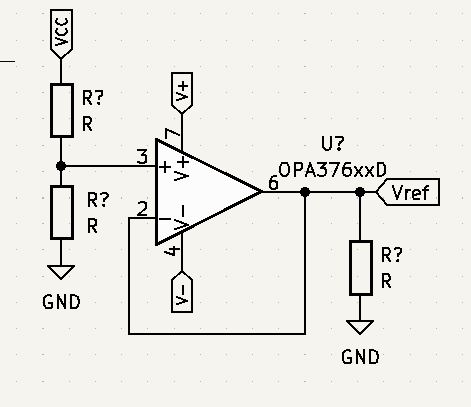
\includegraphics[scale=0.8]{images/Voltagebuffer.jpg}
   \caption{Voltage buffer used to get a stable $V_ref$ amplitude}
    \label{fig:Vbuff}
\end{center}
\end{figure}

\begin{figure} [H]
\begin{center}
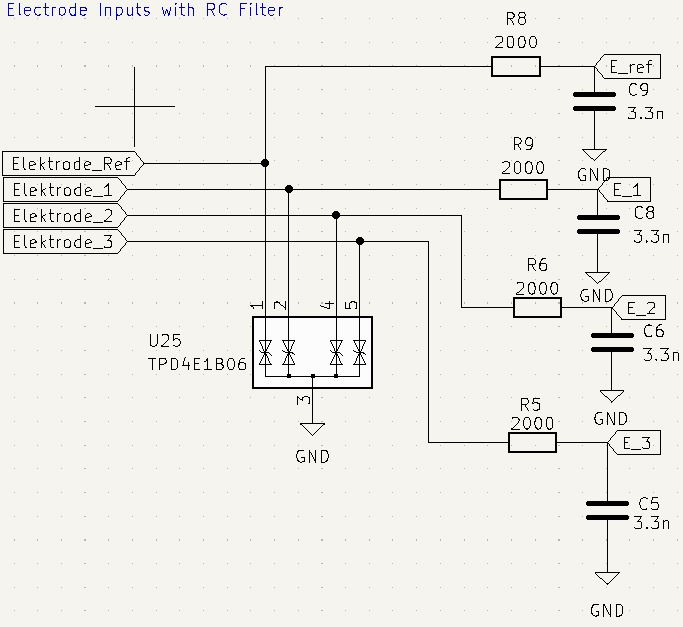
\includegraphics[scale=0.60]{images/Inputcirc.jpg}
   \caption{ESD protection and RC filter used on the electrode input}
    \label{fig:Elecinput}
\end{center}
\end{figure}

\begin{figure} [H]
\begin{center}
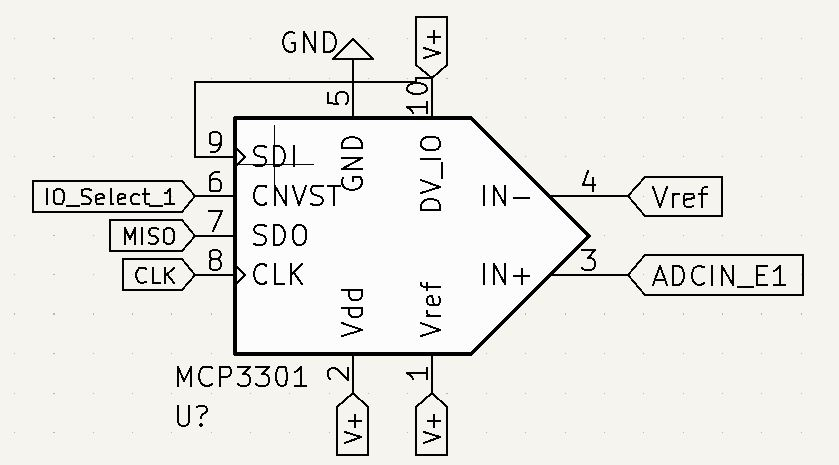
\includegraphics[scale=0.40]{images/ADC_CS_select.jpg}
   \caption{One of the possible ADC configurations using the CS line to select what chip is addressing the SPI line}
    \label{fig:ADC_CS}
\end{center}
\end{figure}
%Could maybe be removed hard to see anything useful
\begin{figure} [H]
\begin{center}
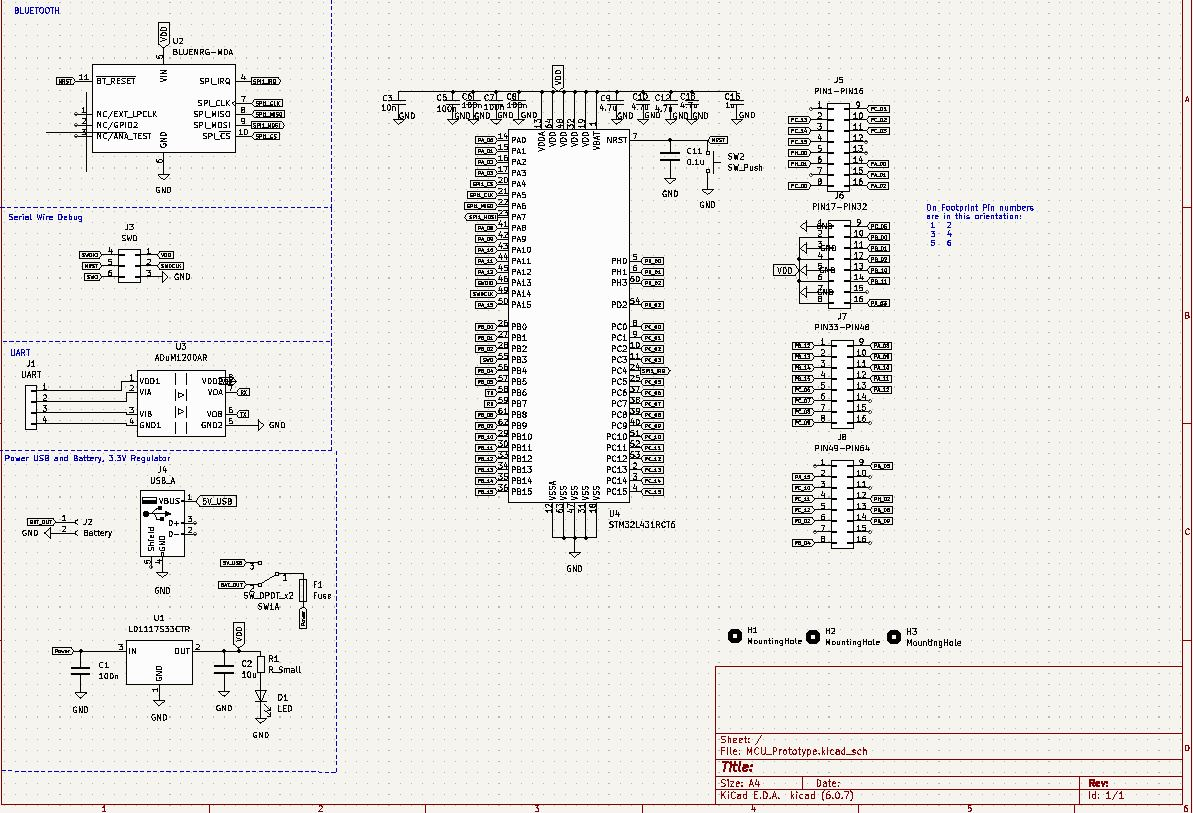
\includegraphics[scale=0.60,angle=-90]{images/FullcircMCU.jpg}
   \caption{The full circuit for the data processing PCB}
    \label{fig:MCUcirc}
\end{center}
\end{figure}

\begin{figure} [H]
\begin{center}
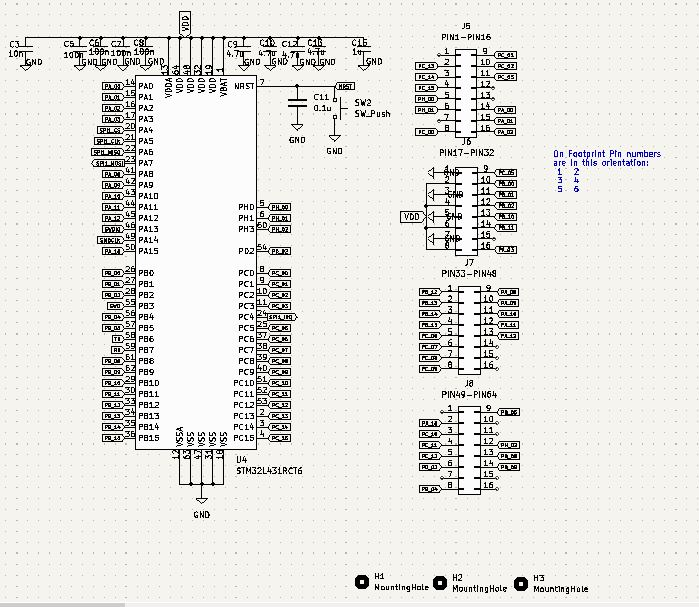
\includegraphics[scale=0.65]{images/MCU.jpg}
   \caption{The MCU configuration with proper decoupling}
    \label{fig:MCU}
\end{center}
\end{figure}

\begin{figure} [H]
\begin{center}
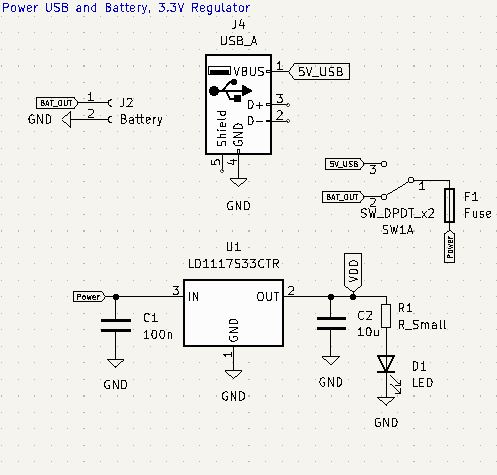
\includegraphics[scale=0.7]{images/Powercirc.jpg}
   \caption{Power circuit for the MCU board with a switch to choose between USB or battery power and a fuse to protect the board from malfunctions.}
    \label{fig:MCUpower}
\end{center}
\end{figure}

\begin{figure} [H]
\begin{center}
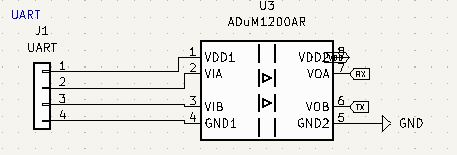
\includegraphics[scale=0.8]{images/UART.jpg}
   \caption{UART configuration with digital isolator}
    \label{fig:MCUuart}
\end{center}
\end{figure}

\begin{figure} [H]
\begin{center}
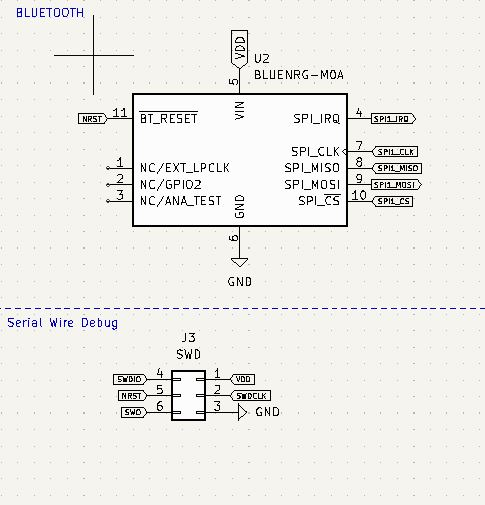
\includegraphics[scale=0.7]{images/BLE_SWD.jpg}
   \caption{Bluetooth configuration and SWD programming pins}
    \label{fig:MCUBLE}
\end{center}
\end{figure}
\subsection{PCBs}
\begin{figure} [H]
\begin{center}
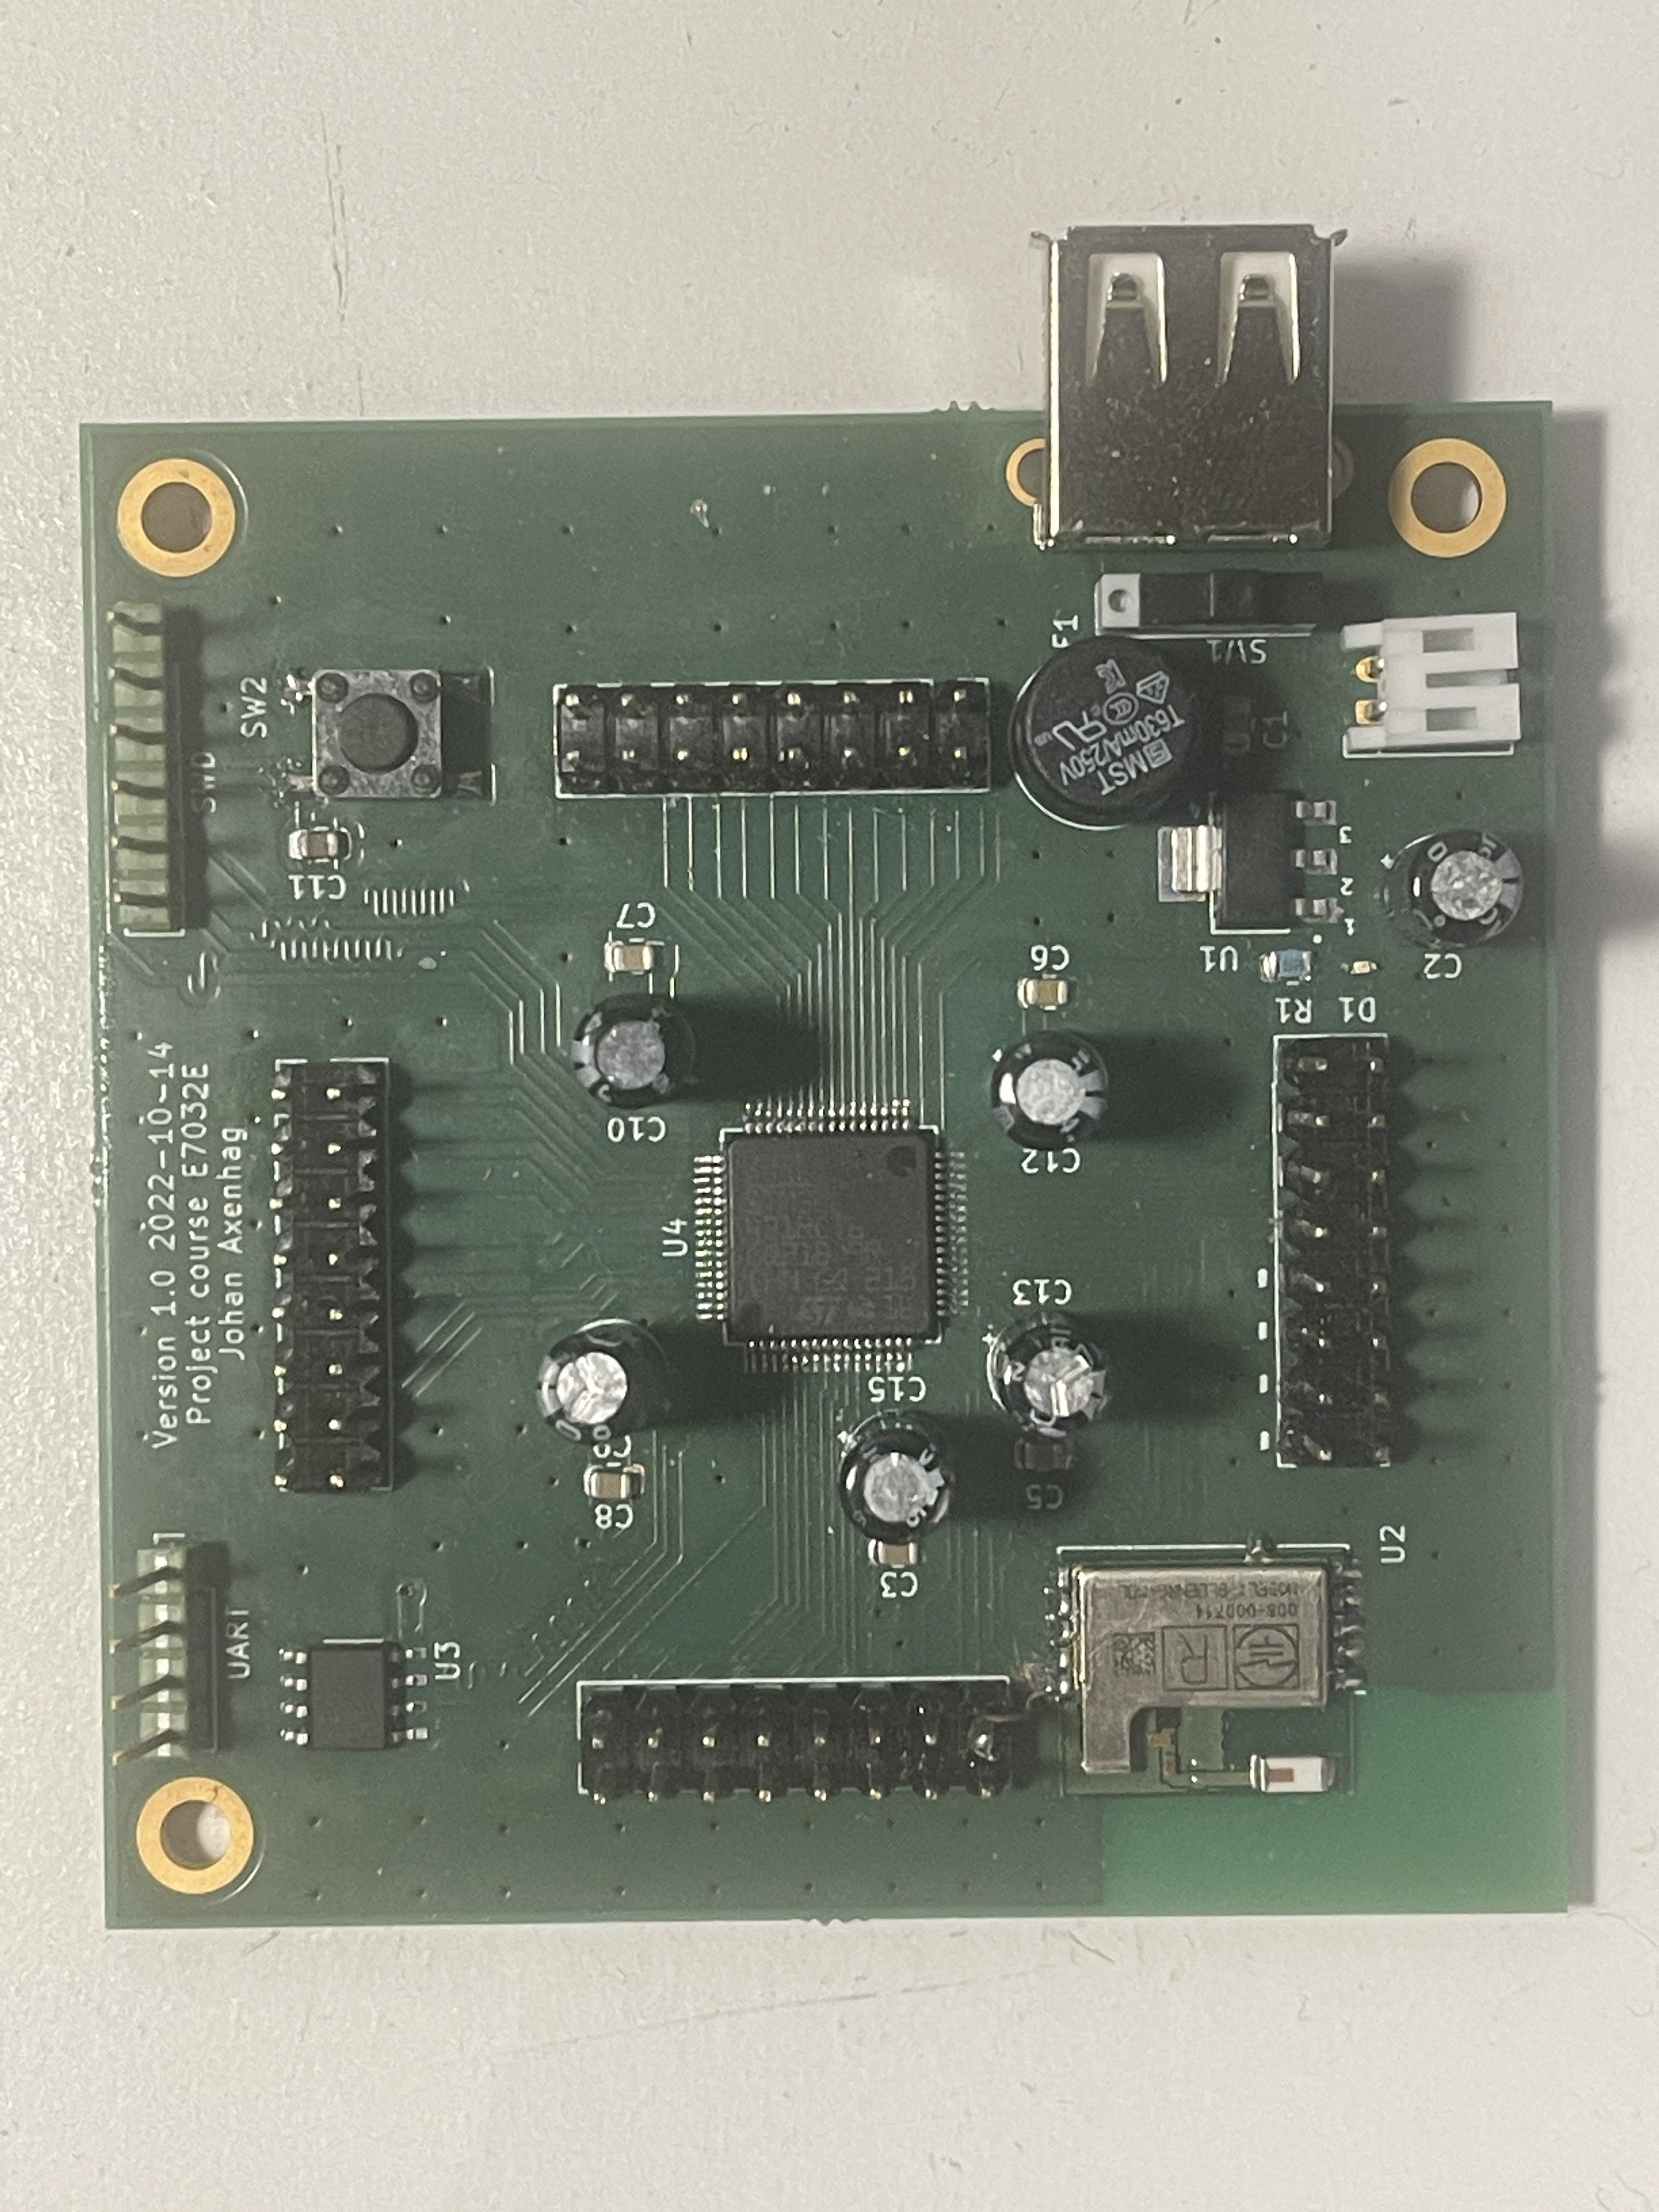
\includegraphics[width=\textwidth]{images/pcb.jpg}
   \caption{The main PCB containing the MCU and Bluetooth module}
    \label{fig:PCBData}
\end{center}
\end{figure}
\section{Components list and cost}
%List of components and costs
Below is a Table presenting the main circuit components and their cost. Since the ADC  design still needs to be thoroughly tested, the choice of ADC is left blank, but the ones bought are in the range of 100 Sek to 700 Sek for an eight channel setup.
\begin{table}[H]
\begin{tabular}{|l|l|l|}
\hline
Components                             & Amount & Cost     \\ \hline
OPA 376                                & 33     & 660 Sek  \\ \hline
Battery 3.7V                           & 1      & 100 Sek  \\ \hline
TPD4E1B06DRLR ESD suppressor           & 3      & 20 Sek   \\ \hline
ADC                                    & 8      & -        \\ \hline
MCU                                    & 1      & 100 Sek  \\ \hline
Voltage regualtro                      & 1      & 30 Sek   \\ \hline
UART isolator                          & 1      & 20 Sek   \\ \hline
BlueNRG                                & 1      & 100 Sek  \\ \hline
PCB                                    & 1      & 370 Sek  \\ \hline
Misc (Resistor, Capacitors, LEDs, etc) & -      & 100 Sek  \\ \hline
Total                                  &        & 1500 Sek \\ \hline
\end{tabular}
\end{table}
\newpage
%%%%%%%%%%%%%%%%%%%%%%%%%%%%%%%%%%%%%%%%%%%%%%%%%%%%%%%%%%%%%%
% -                    Bibliography                        - %
%%%%%%%%%%%%%%%%%%%%%%%%%%%%%%%%%%%%%%%%%%%%%%%%%%%%%%%%%%%%%%
\printbibliography % - Here we say that the bibliography should be printed. The section title "References" is printed automatically.

% I denna del anges de källor du använt i ditt arbete. Ange bara de viktigaste och alla
% referenser i listan måste vara refererade till i texten. I referenslistan får det inte
% förekomma någon referens som är ``allmänt bra att ha'' utan endast de referenser som
% författaren själv använt. Alla referenser ska refereras till i texten.
% OBS! använd originalreferenser. Undvik referenser till webbsidor eftersom de kan försvinna/ändras.
% Ett av de vanligaste är att man skriver
% författarnamnet och sedan referensens publikationsår - det s.k. Harvard systemet.
% Exempel: ... även funnet av Charpak (1983)
% Är det två eller flera författare brukar man skriva
% Två författare: ... även funnet av Charpak och Öqvist (1983).
% Flera författare: ... även funnet av Charpak et al. (1983).
% ( et al. är latin (et alii) och betyder ``och andra'').
% Ett annat sätt att ange en referens är att numrera referenserna i den ordning de dyker
% upp i texten och sortera referenslistan i nummerordning.
% Exempel: ... som Öqvist [3] har funnit, och referensen Öqvist dyker då upp som nummer tre i referenslistan.
% En guide för referenser finns här: http://libguides.ltu.se/skrivaoreferera
% hej

\end{document}


